\chapter{Related Work}
\label{chapter:Related_Work}

\begin{figure}[h!]
  \caption{A picture of a gull.}
  \centering
    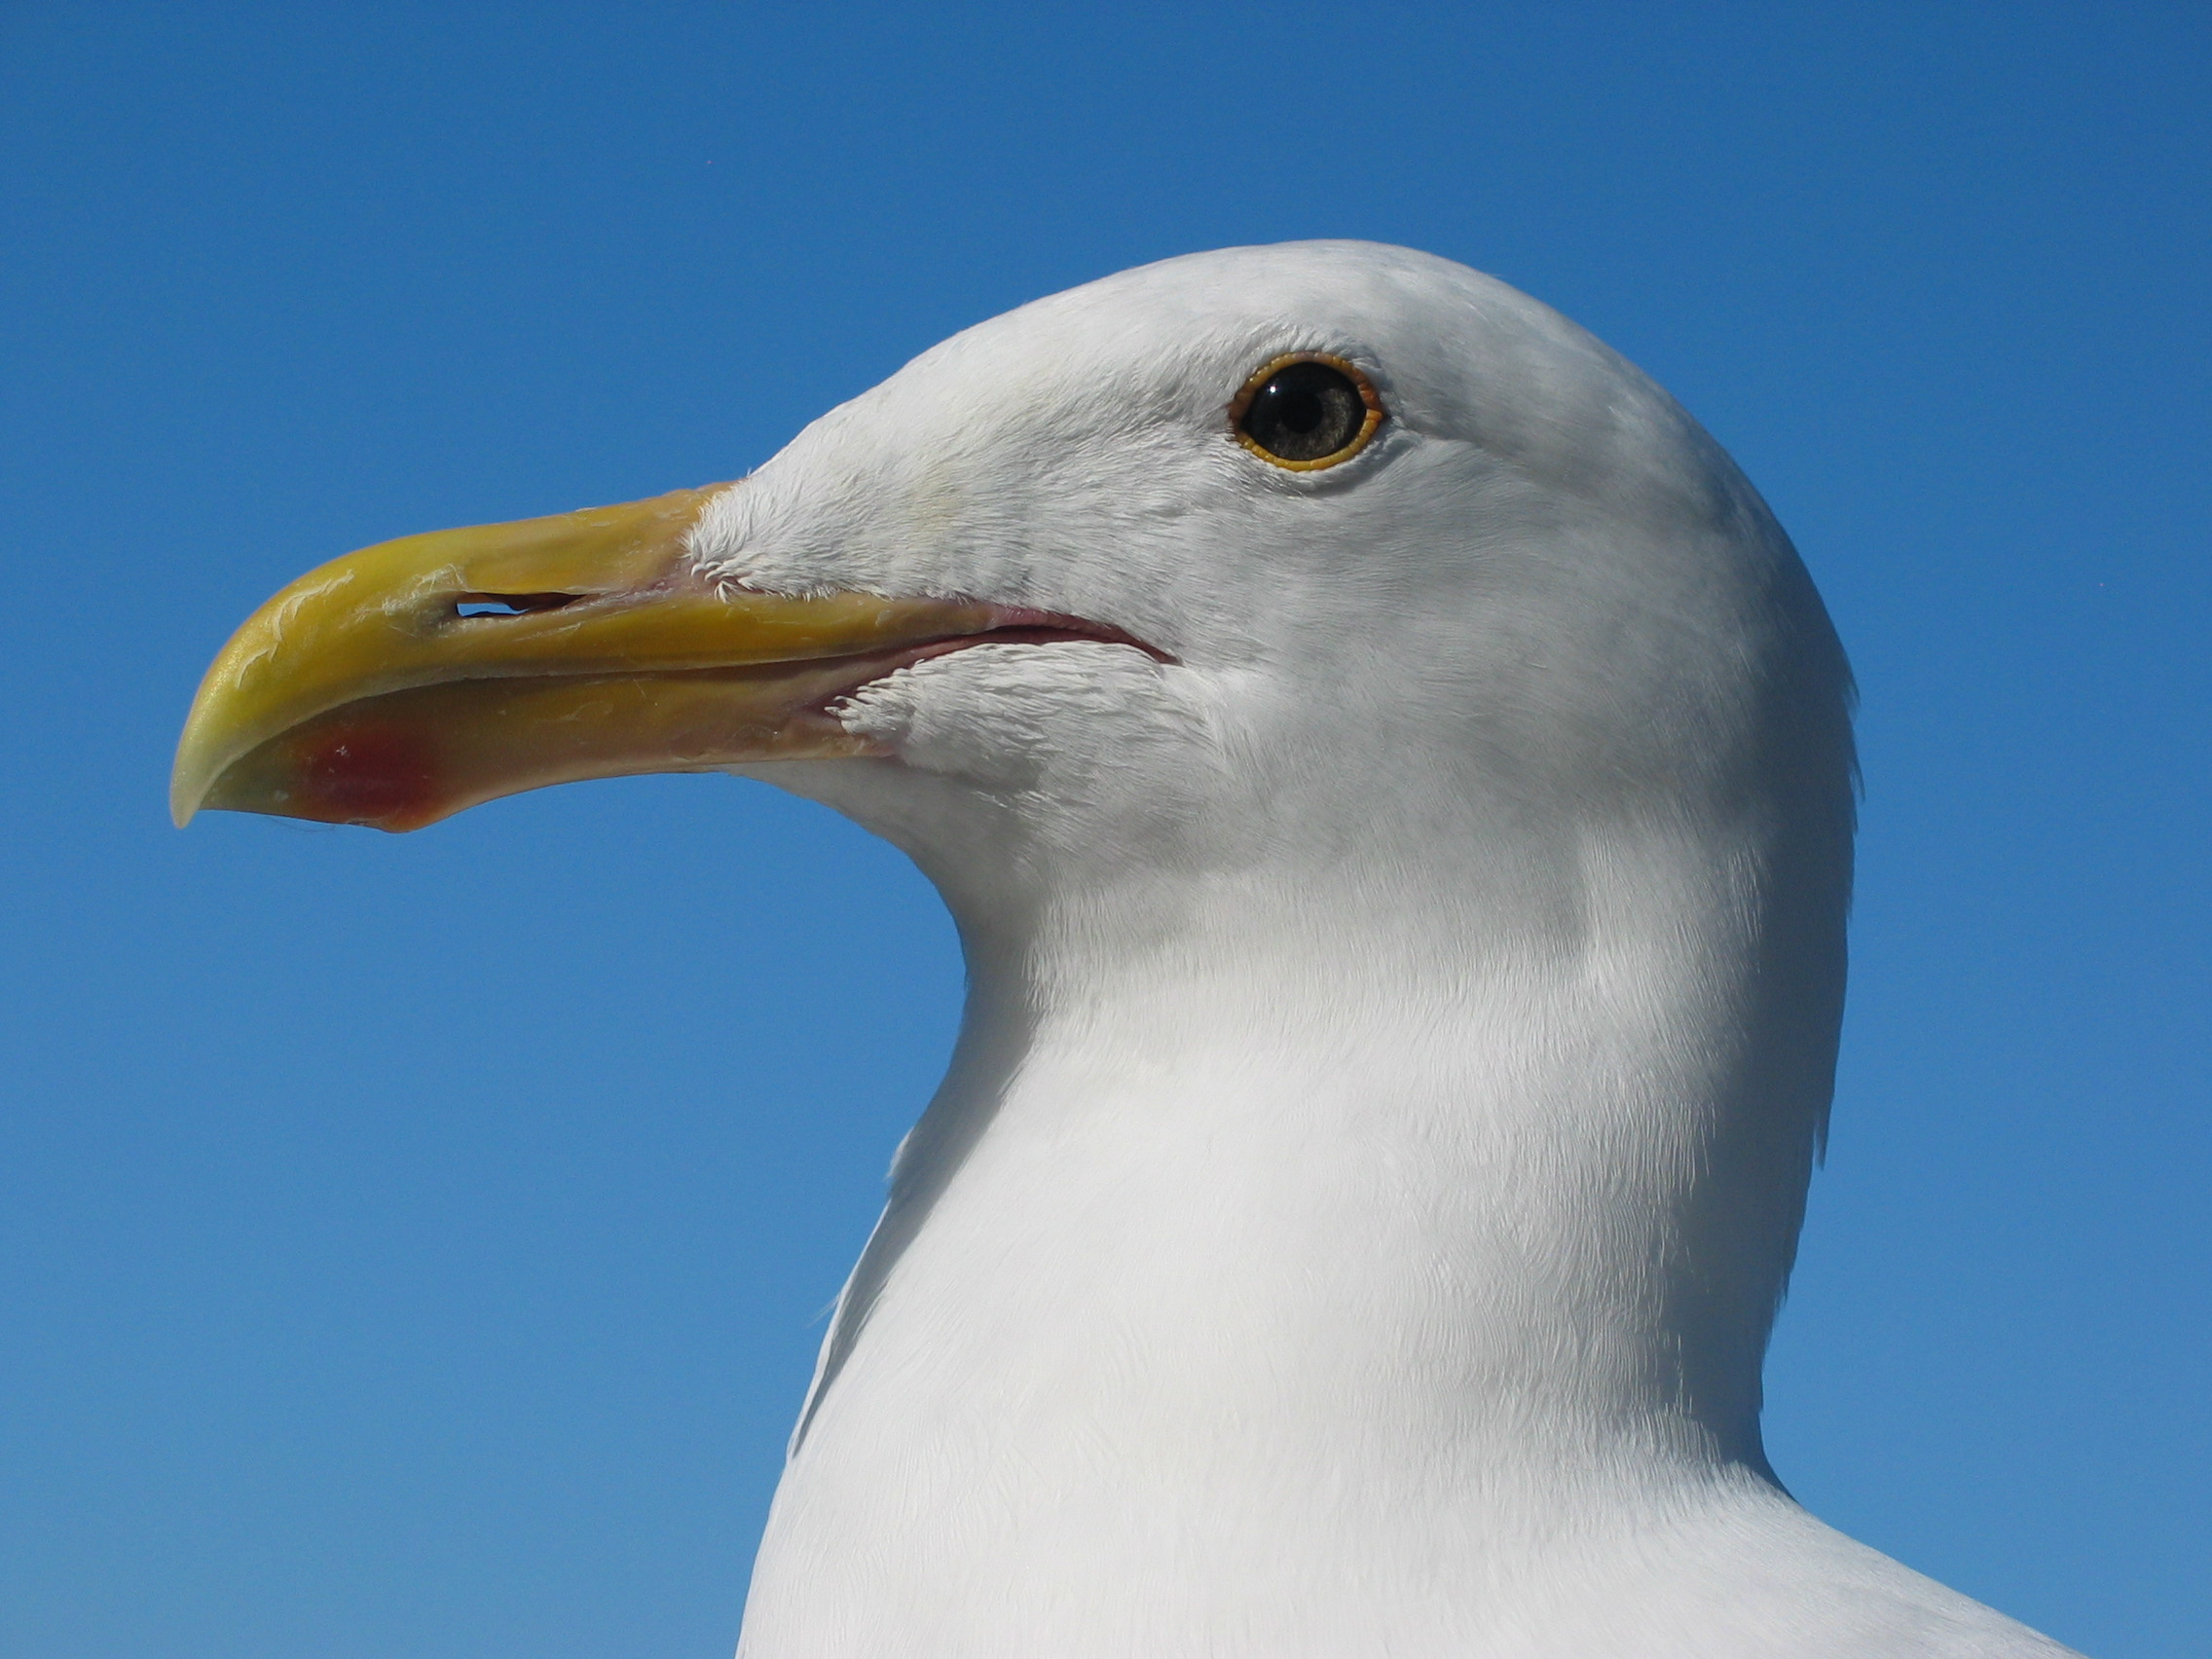
\includegraphics[width=0.8\textwidth]{chapters/images/gull}
\end{figure}

\section{3D geometry}

Yes  - do coordinate systems, transformations, notation
Brief description of SE(3) and SO(3)

\section{Camera Models}

In order to utilise a camera as a sensor, a mapping between camera coordinates and world coordinates
needs to be derived.  To achieve this mapping a model of the camera is required.  This section will
cover all the different types of cameras used in this work and corresponding camera models for
each. 

\subsection{Pinhole Camera Model}

\begin{figure}[h!]
  \caption{Pinhole Camera}
  \centering
    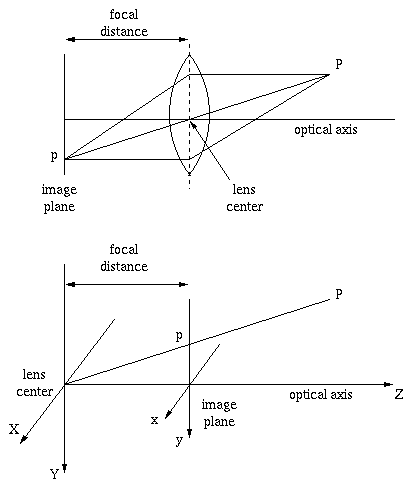
\includegraphics[width=0.5\textwidth]{chapters/images/pinhole_camera}
\end{figure}

\subsection{Stereo Camera}

\subsection{Omni-directional Camera}

\subsection{Flir}

\section{Computer Vision Basics}

\subsection{Feature point detection and extraction}

SIFT - Scale Invariant something whatever
SURF - Speeded up robost something

\subsection{RANSAC}

\subsection{Geometry estimation}

\subsubsection{5 point algorithm}
Umeyama/horn

\subsubsection{Point triangulation}

\subsubsection{Stereo pose estimation}

\section{Place Recognition}

Bag of words

\section{Visual SLAM}
Not sure about this one.  It will be covered extensively when I talk about ScaViSLAM

\subsection{Keyframe SLAM}

\subsection{Graph SLAM}
